\chapter{Experiments and Results}\label{ch:experiments}
This section will present the experiments carried out in the different parts of SemReBot2 as well as a full system test. For a discussion around the results, see Section \ref{ch:discussion}. The experiments aim to highlight the advantages and disadvantages of the different model sizes, and each subsection will present the key findings for each part of SemReBot2. A full description of the test sets and results can be found in Appendix \textcolor{red}{X}. 

The experiments are primarily targeted at the specific use case of SemReBot2. Creators of models and packages used in SemReBot2 have conducted their own experiments for general purpose use, and the reader is encouraged to read the official papers of Whisper\cite{radford_robust_2022}, Mistral\cite{jiang_mistral_2023}, POPF\cite{coles_forward-chaining_2021} and PlanSys2\cite{martin_plansys2_2021} respectively for general performance experiment results.

\section{Whisper}\label{sec:Whisper_experiments}
The experiments conducted on Whisper were performed to compare the performance of different model sizes and to determine whether loading models with flash attention increased or decreased performance. The chosen metrics were WER, RTF, allocated memory during inference, and inference time.

The test set consists of ten audio files with a corresponding reference text. The audio files are news segments with a duration of 123 seconds to 824 seconds downloaded from Rev.com\cite{revcom_transcript_2024}, accompanied by a transcribed text.

The key results can be seen in Figure \ref{fig:whisper_avg}.

\begin{figure}[h]
    \centering
    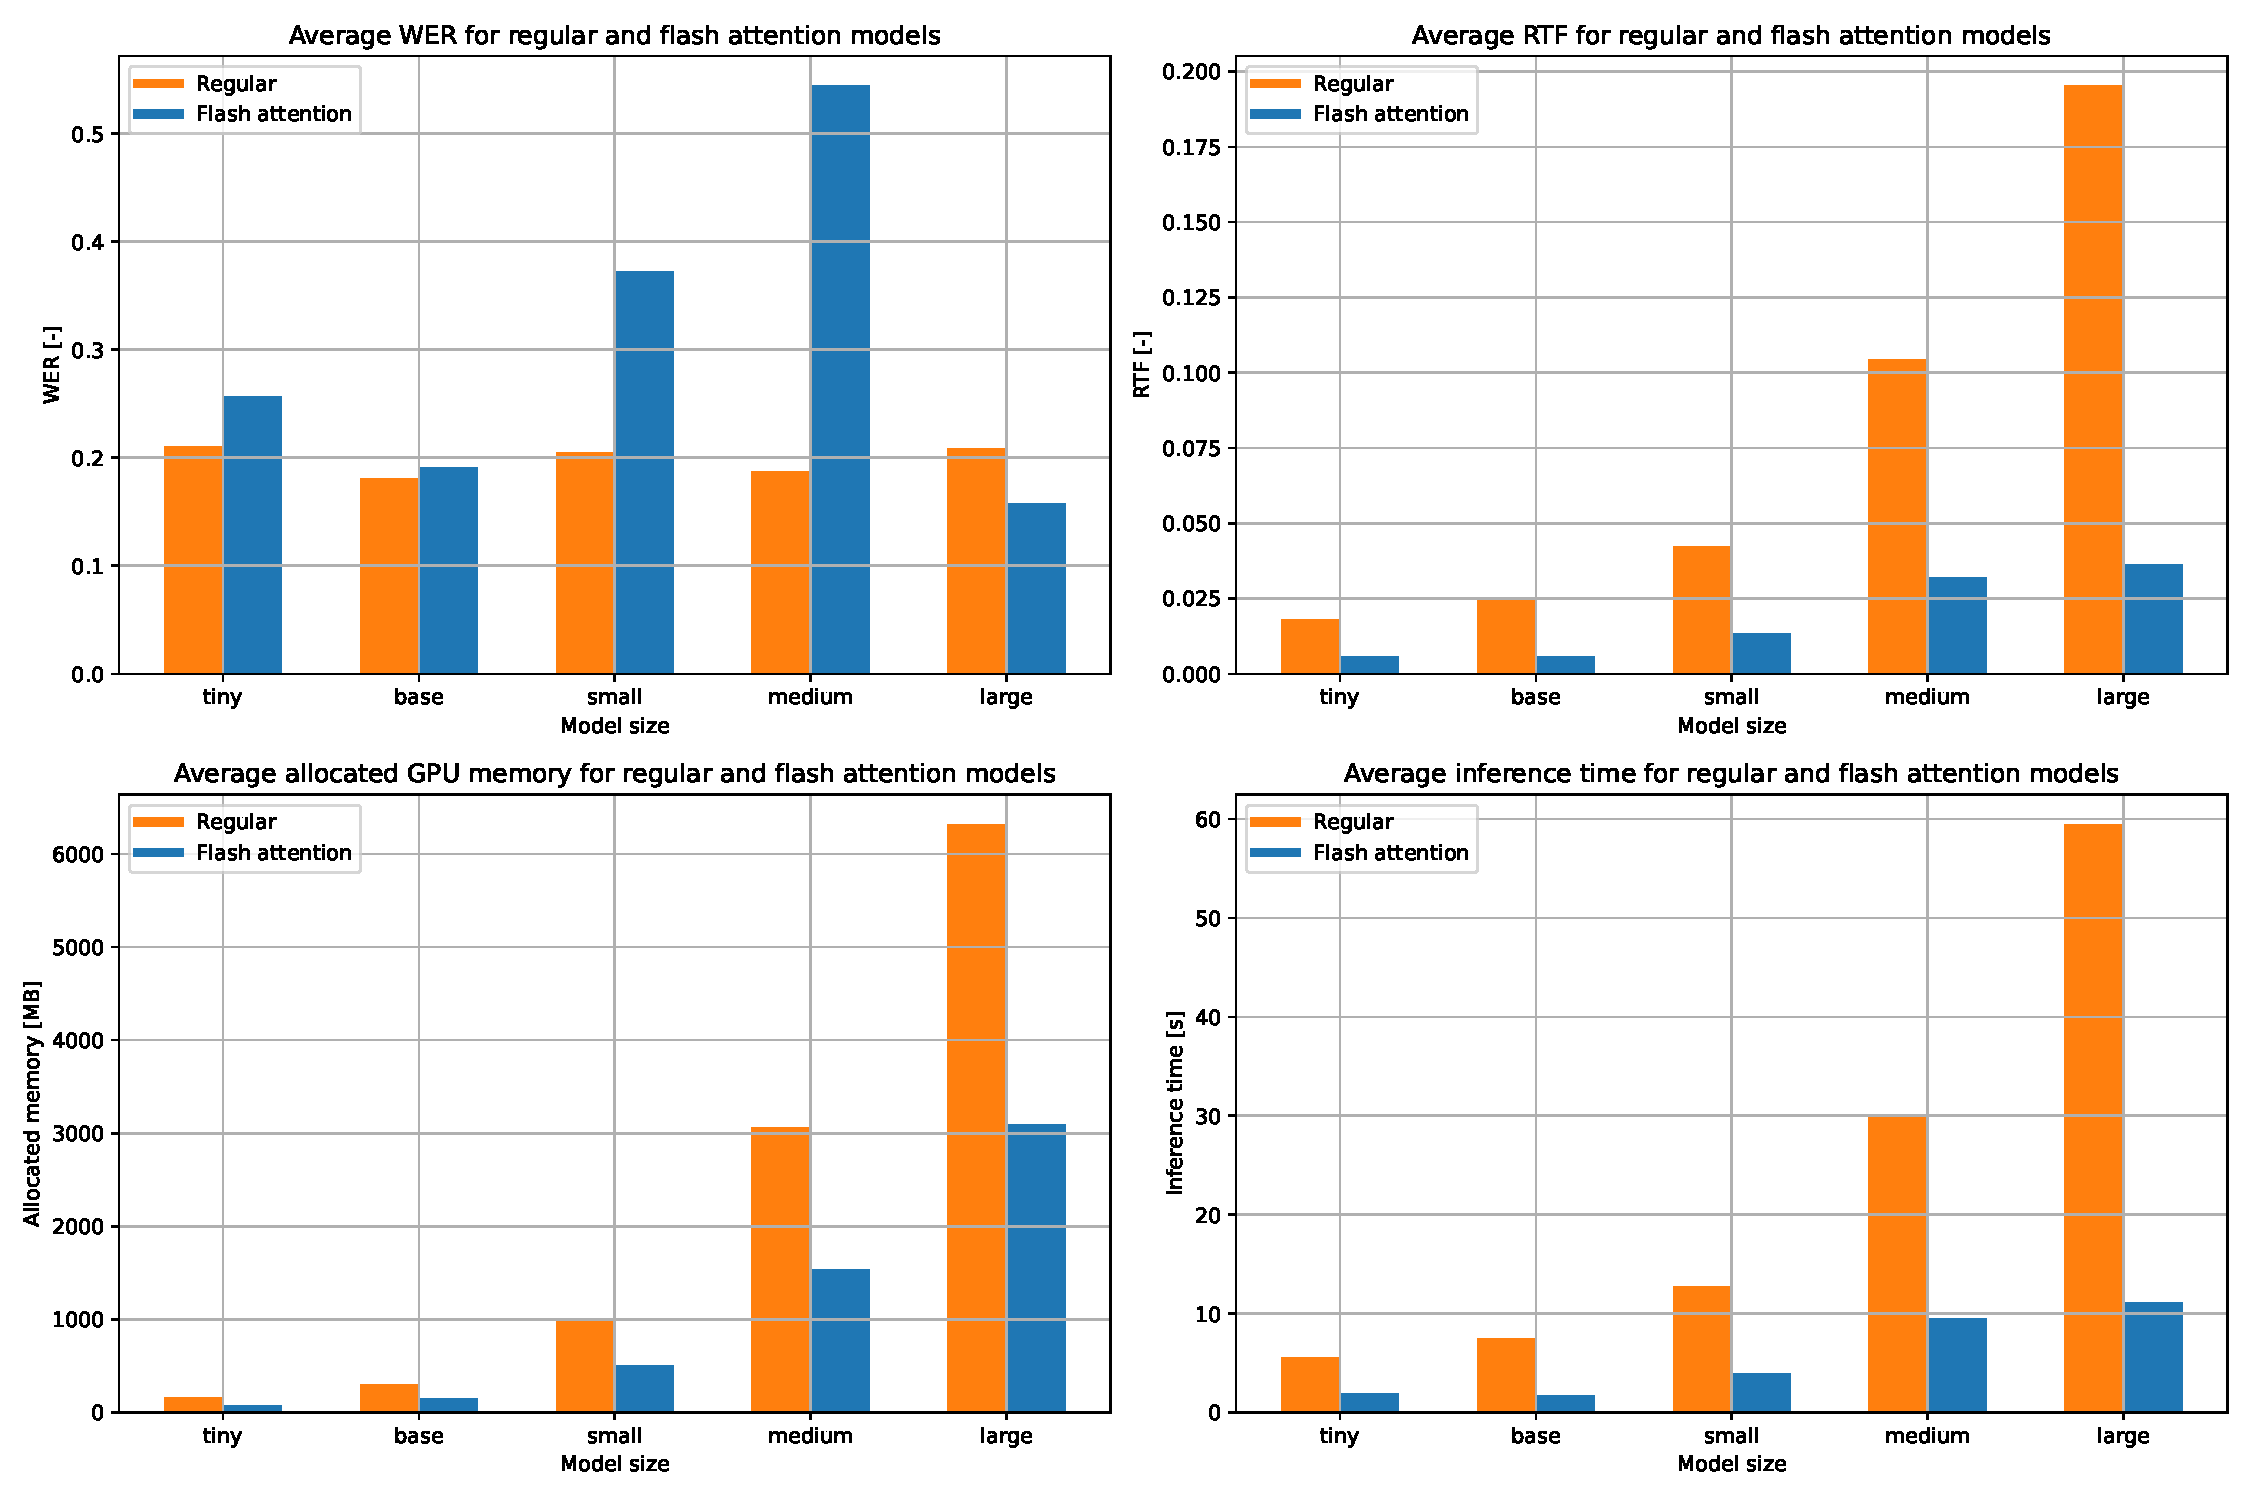
\includegraphics[width=\textwidth]{figures/avg.pdf}
    \caption[Whisper experiment results]{Comparison of Whisper model sizes loaded with flash attention and not. Measured metrics are WER (top left), RTF (top right), allocated memory during inference (bottom left) and average inference time (bottom right).}
    \label{fig:whisper_avg}
\end{figure}

\section{Mistral}\label{sec:Mistral_experiments}
Experiments conducted on Mistral were specific to the PDDL domain and the desired output format used in SemReBot2. We created two test sets where Mistral was given a PDDL domain with types and predicates available, as well as a natural language command.

\subsection{Test sets}
In test set 1, containing ten elements, each element consists of a domain extracted from the Github repository \verb|pddl-generators| by the AI-Planning community\cite{favorito_ai-planningpddl-generators_2024}\footnote{This repository contain domains and problems used to generate benchmarks for the International Planning Competition.}. We then accompany each domain with a natural language command and a solution containing the correct instances, predicates, and goals in the correct format as SemReBot2 expects. An element of test set 1 can be seen in Table \ref{tab:test_set}

In test set 2, all eleven elements contain the same PDDL domain, which is the same domain as in the simulated environment, but different accompanying natural language commands and solutions. This test set is specific to the SemReBot2 use case.

\subsection{Shot sets}
For each test set, we created one or two sets that we call "shot sets". For test set 1, we created two shot sets, shot set 1 and shot set 2, with PDDL domains from \verb|pddl-generators| (but not the same as in test set 1), containing 32 elements with an accompanying natural language command and an output. The difference between shot set 1 and shot set 2 is that shot set 1 is unlabelled, while shot set 2 is labelled. That is, all the outputs in shot set 1 are correct, while every other output in shot set 2 is correct or wrong. So, shot set 2 contains an extra marker \verb|label| which is either \verb|correct| or \verb|wrong|. An element of shot set 2 can be seen in Table \ref{tab:labeled_shot_set}.

For test set 2, we used the same shot set as test set. However, if Mistral was running a test on element \verb|i| in test set 2, the shot set would contain all the previous elements in test set 2 as shots. This means that shot set 3 contains ten elements (\verb|len(test_set_2) - 1|).

\subsection{System prompts}\label{ssec:system_prompt}
For all the tests we ran, we created three different system prompts. A system prompt represents a chat history between a user and the assistant (read Mistral). All three system prompts explain what role Mistral has, its goal, and show one example of domain, natural language command, and expected output. The difference between the three is the length and the amount of detail Mistral is given. The prompts range between what we call "short and precise", "medium detailed", and "long and detailed". Table \ref{tab:system_prompt} shows the short and precise system prompt.

\subsection{Tests}
The first test was performed to spot performance differences between a fine-tuned model for "SemReBot2 use" and zero-, one-, and few-shot prompting.

\subsection{Fine-tuned model}

\subsection{Pre-prompted model}
For the pre-prompted model tests, we ran three different tests:

\begin{itemize}
    \item Generic PDDL domain without labels
    \item Generic PDDL domain with labels
    \item Specific PDDL domain without labels
\end{itemize}

Every test was set up the same way: We first load the model into memory, extract one element from the test set, extract zero or more elements from the shot set depending on the number of iterations, run inference, and record the output before writing it to a file for storage. For all elements in a test set, we ran through all the elements in a shot set. This means that we recorded \verb|length(test_set)*length(shot_set)| number of test runs for each test set. We ensured that there was no information from previous test runs in Mistral by deleting and reloading the model before every inference run. See Appendix \textcolor{red}{X} for the model parameters used during the testing.

\begin{algorithm}\label{alg:mistral_test}
    \caption{Testing Mistral}
    \begin{algorithmic}[1]
        \State Load shot set, test set and system prompts
        \For{\textbf{each} test \textbf{in} test set}
            \For{\textbf{each} system prompt \textbf{in} system prompts}
                \For{\textbf{each} shot \textbf{in} shot set}
                    \State messages := system prompt + shot + test
                    \State Load model into memory
                    \State Perform model inference on messages
                    \State Write metric results to file
                    \State Delete model from memory and release resources
                \EndFor
            \EndFor
        \EndFor
    \end{algorithmic}
\end{algorithm}

In all tests, we measured the inference time, allocated GPU memory during inference, model input size, and Mistral output compared to the solution. For the output, we used four metrics: precision, recall, F1 score, and our own defined metric accuracy. Accuracy is computed by comparing the output instances, predicates, and goals compared to the solution instances, predicates, and goals. The evaluation metric is subdivided
into four distinct categories: $\text{accuracy}_{instances}$, $\text{accuracy}_{predicates}$, $\text{accuracy}_{goals}$ and $\text{accuracy}_{total}$.

\begin{equation}\label{eq:mistral_accuracy_metric}
    \text{accuracy}_{type}(\text{domain}, \text{command})=
    \begin{cases}
        1 & \text{if } \text{output}_{type} = \text{solution}_{type} \\
        0 & \text{otherwise}
    \end{cases}
\end{equation}
where $type = (instances, predicates, goals)$.

As seen in Equation \ref{eq:mistral_accuracy_metric}, each $type$ category employs a binary classification approach, in which the precision is deemed "correct" iff the output is exactly like the solution, disregarding variations in variable names. The total accuracy is then defined as

\begin{equation}\label{eq:mistral_total_accuracy_metric}
    \text{accuracy}_{total}=\text{accuracy}_{instances}\times \text{accuracy}_{predicates}\times \text{accuracy}_{goals}
\end{equation}

\subsubsection{Generic PDDL domain test results}
The generic PDDL domain tests, we evaluated Mistral's performance on unlabelled and labelled shot sets. The test set and the system prompt were the same for all tests.

An overview of the test results can be seen in Figure \ref{fig:mistral_trend_lines}, Figure \ref{fig:mistral_inf_time} and Figure \ref{fig:mistral_heatmaps}. The figures show the trend line of the precision, recall, and F1 score, a scatter plot of the inference time, and a heatmap of $\text{accuracy}_{total}$, respectively, comparing unlabelled and labelled data.

\begin{figure}[h]
    \centering
    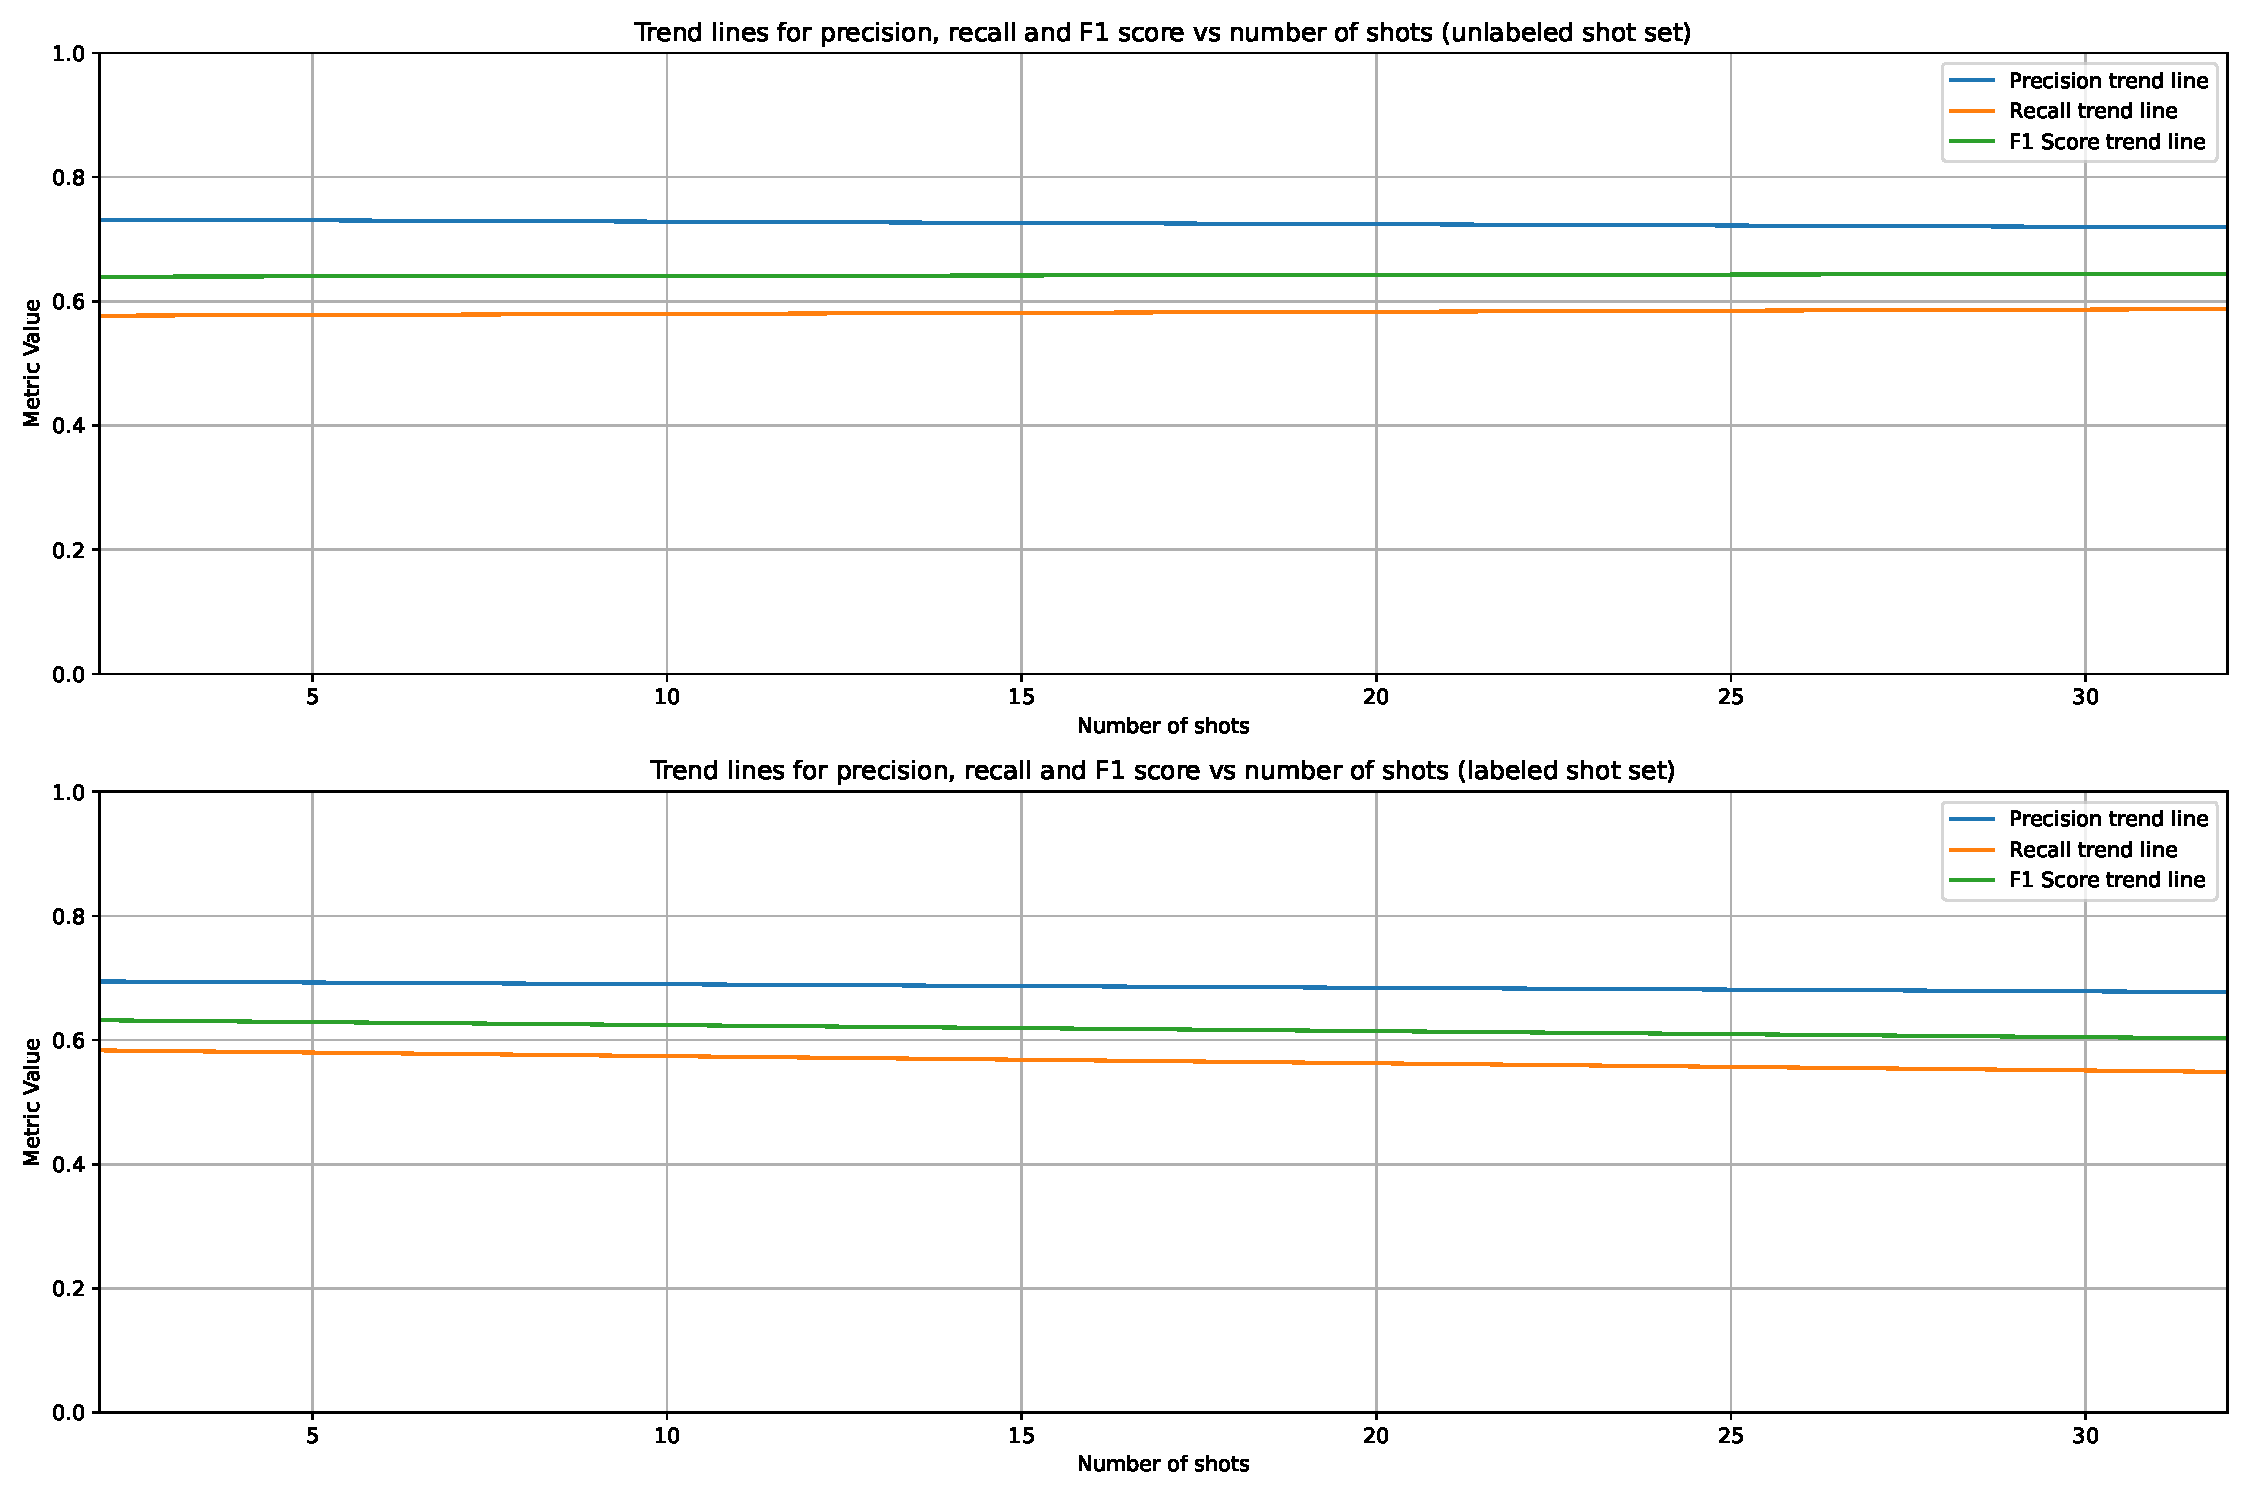
\includegraphics[width=\textwidth]{figures/ul_trend_lines.pdf}
    \caption[Mistral all metrics trend lines]{Trend lines for precision, recall and F1 score for Mistral on unlabelled and labelled data.}
    \label{fig:mistral_trend_lines}
\end{figure}

\begin{figure}[h]
    \centering
    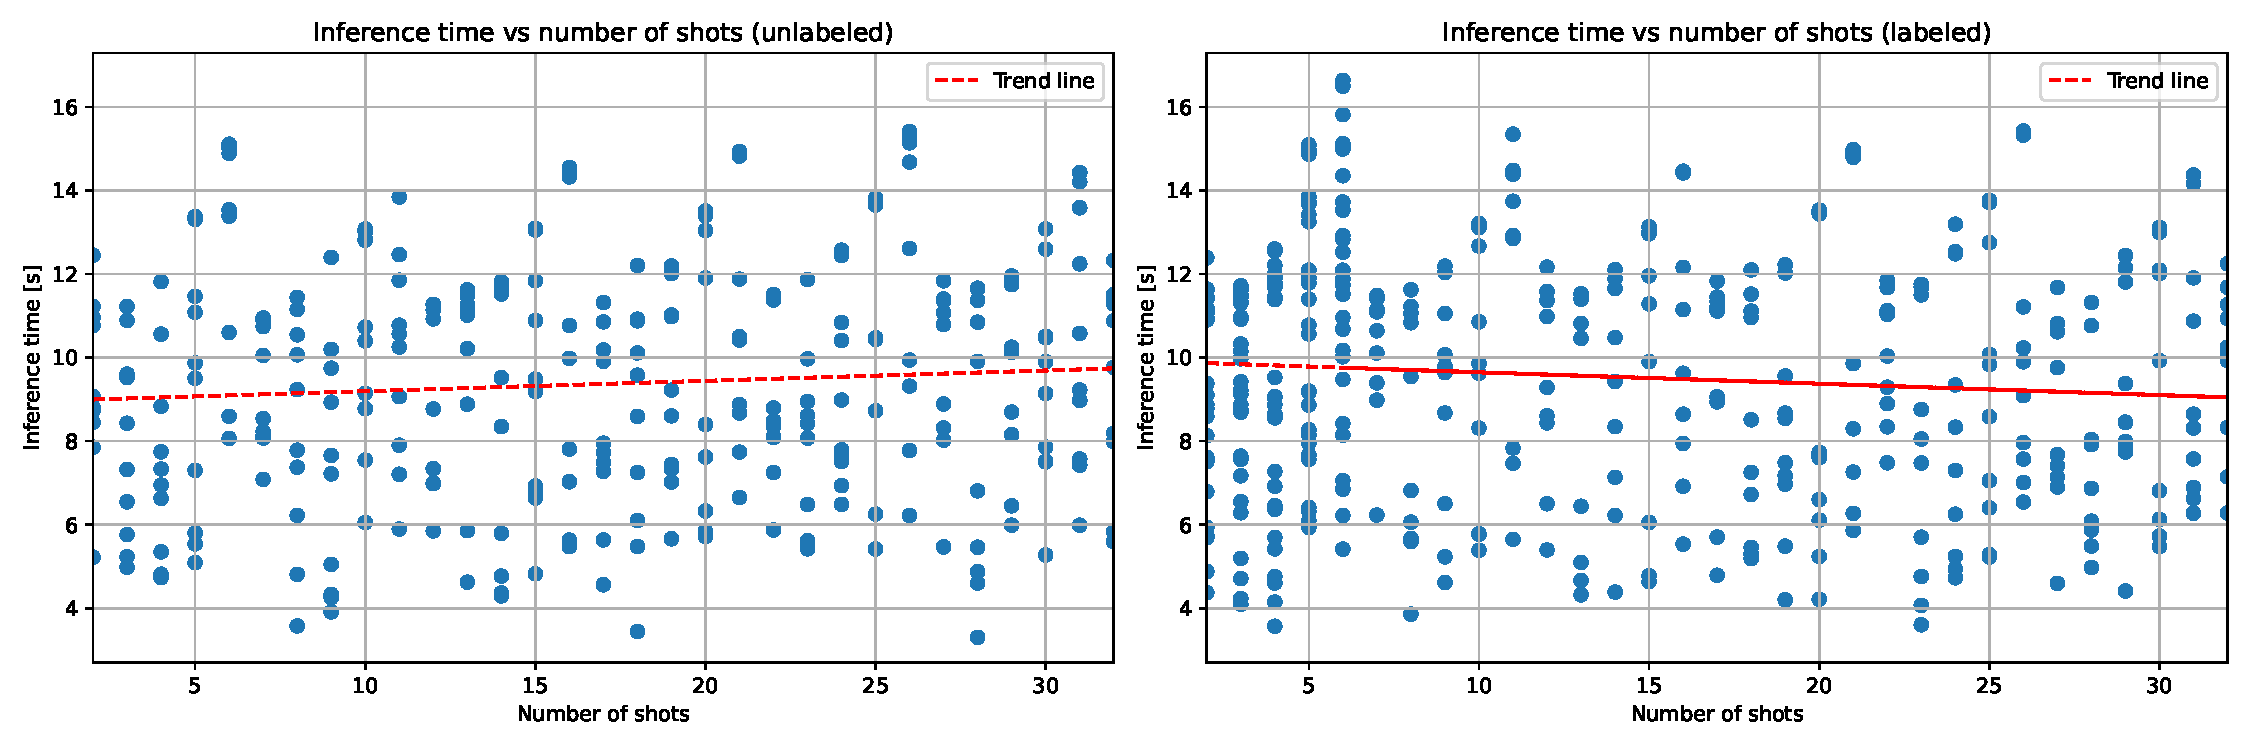
\includegraphics[width=\textwidth]{figures/ul_inf_time.pdf}
    \caption[Mistral inference time]{A scatter plot of the inference time at each test. The red, stippled, line shows the trend line of all recorded inference times.}
    \label{fig:mistral_inf_time}
\end{figure}

\begin{figure}[h]
    \centering
    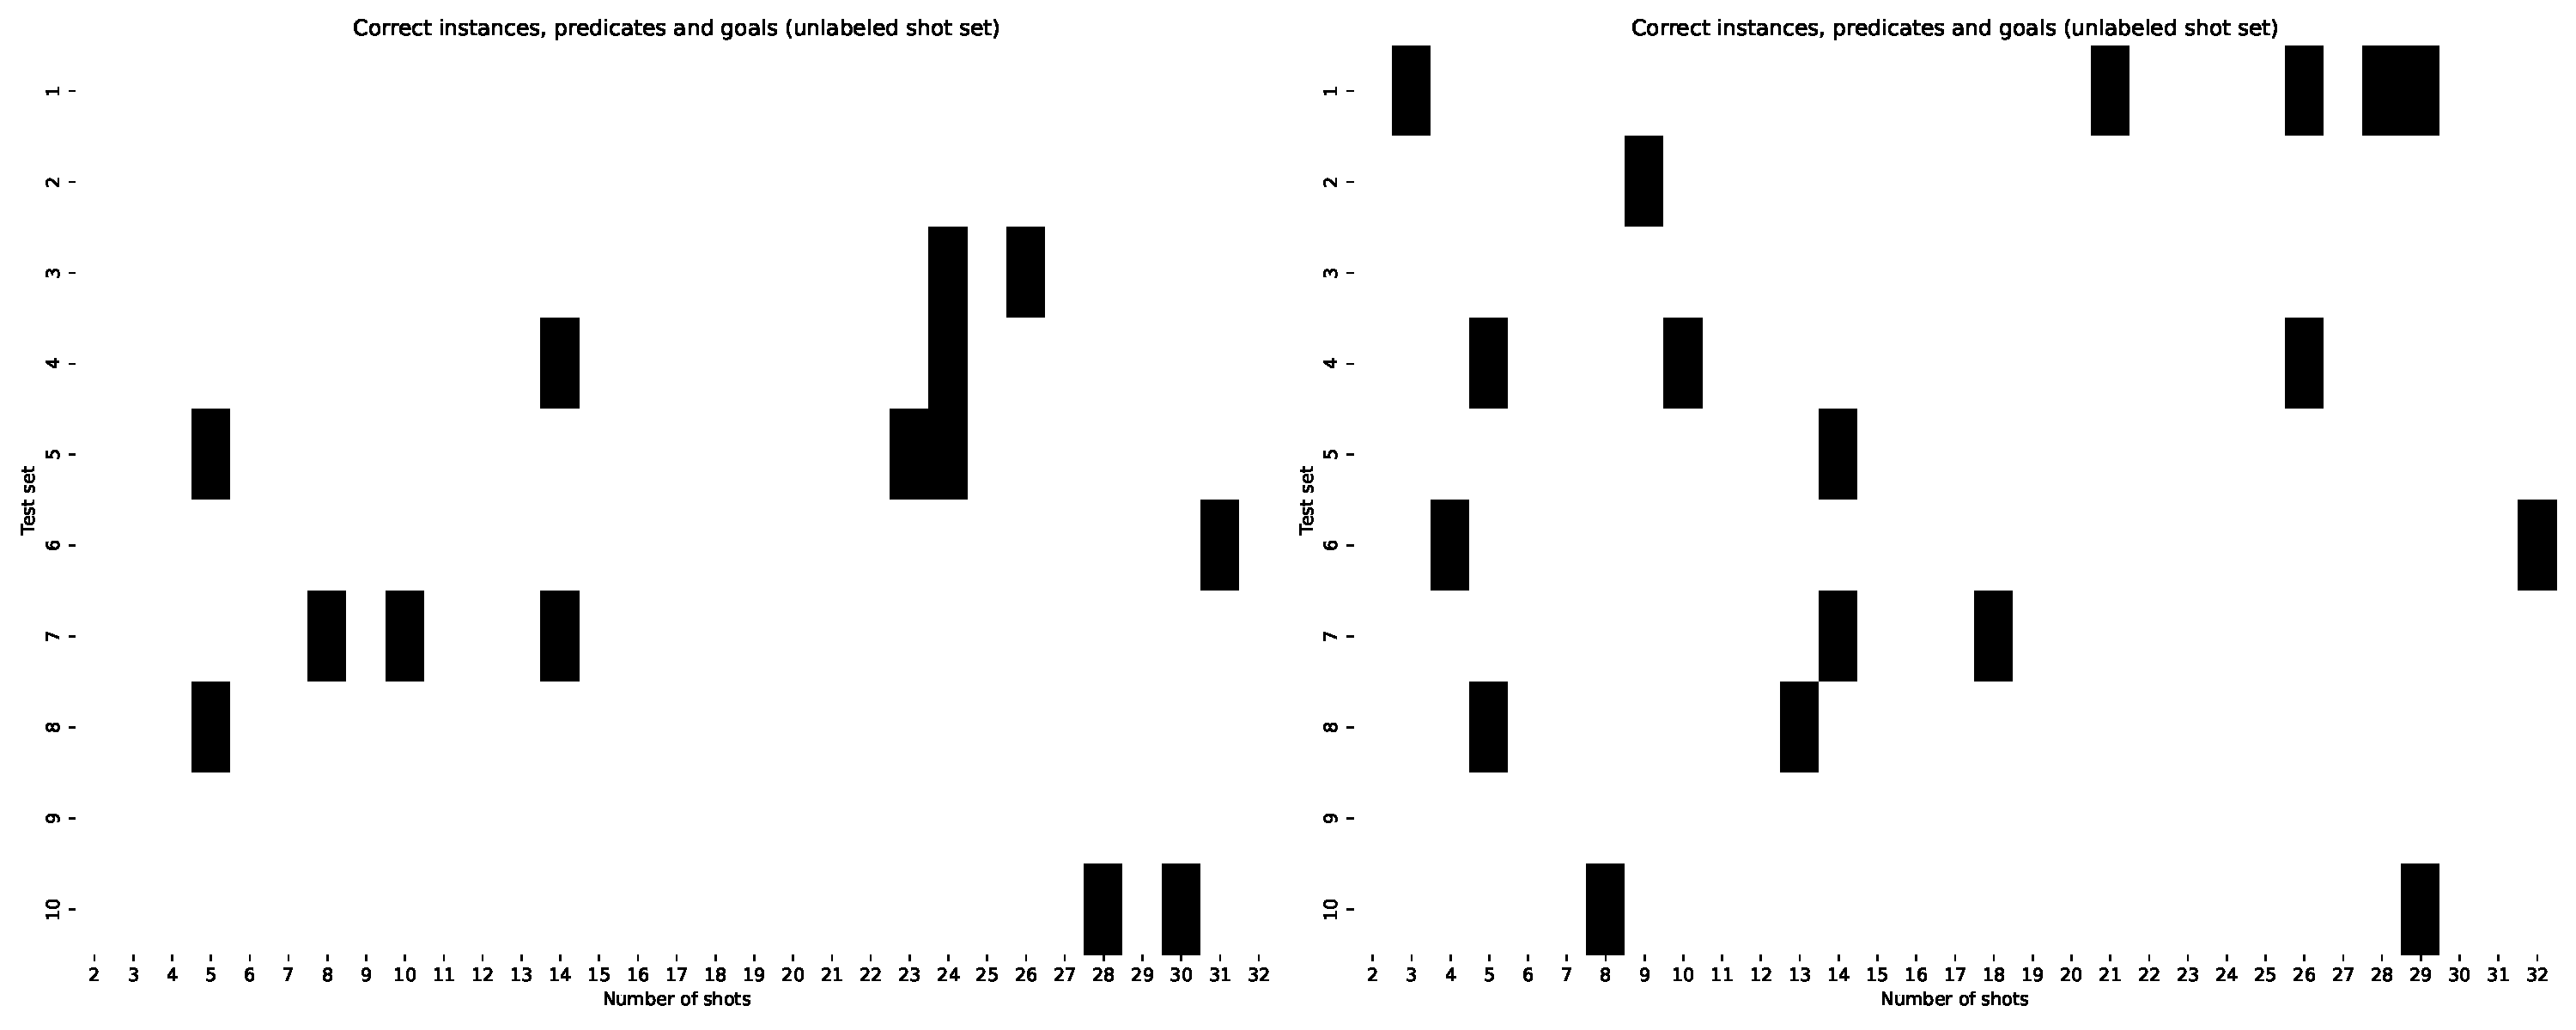
\includegraphics[width=\textwidth]{figures/ul_heatmaps.pdf}
    \caption[Mistral $\text{accuracy}_{total}$ heatmaps]{Heatmaps showing the $\text{accuracy}_{total}$ at each test set for number of shots.}
    \label{fig:mistral_heatmaps}
\end{figure}

\subsubsection{Specific PDDL domain test results}
For the specific PDDL domain tests, we evaluated Mistral's performance for three different prompts, with and without generated knowledge on test set 2. The generated knowledge was given as everything in the domain that was true when Mistral is initiated, see Table \ref{tab:generated_knowledge} in Appendix \textcolor{red}{X}.

An overview of the test results can be seen in Figure \ref{fig:specific_all_metrics_trend}, Figure \ref{fig:specific_avg_inf_time} and Figure \ref{fig:specific_heatmap}. The figures show the trend line of the precision, recall, and F1 score, the average inference time, and a heatmap of $\text{accuracy}_{total}$, respectively, for all prompts, with and without generated knowledge. 

\begin{figure}[h]
    \centering
    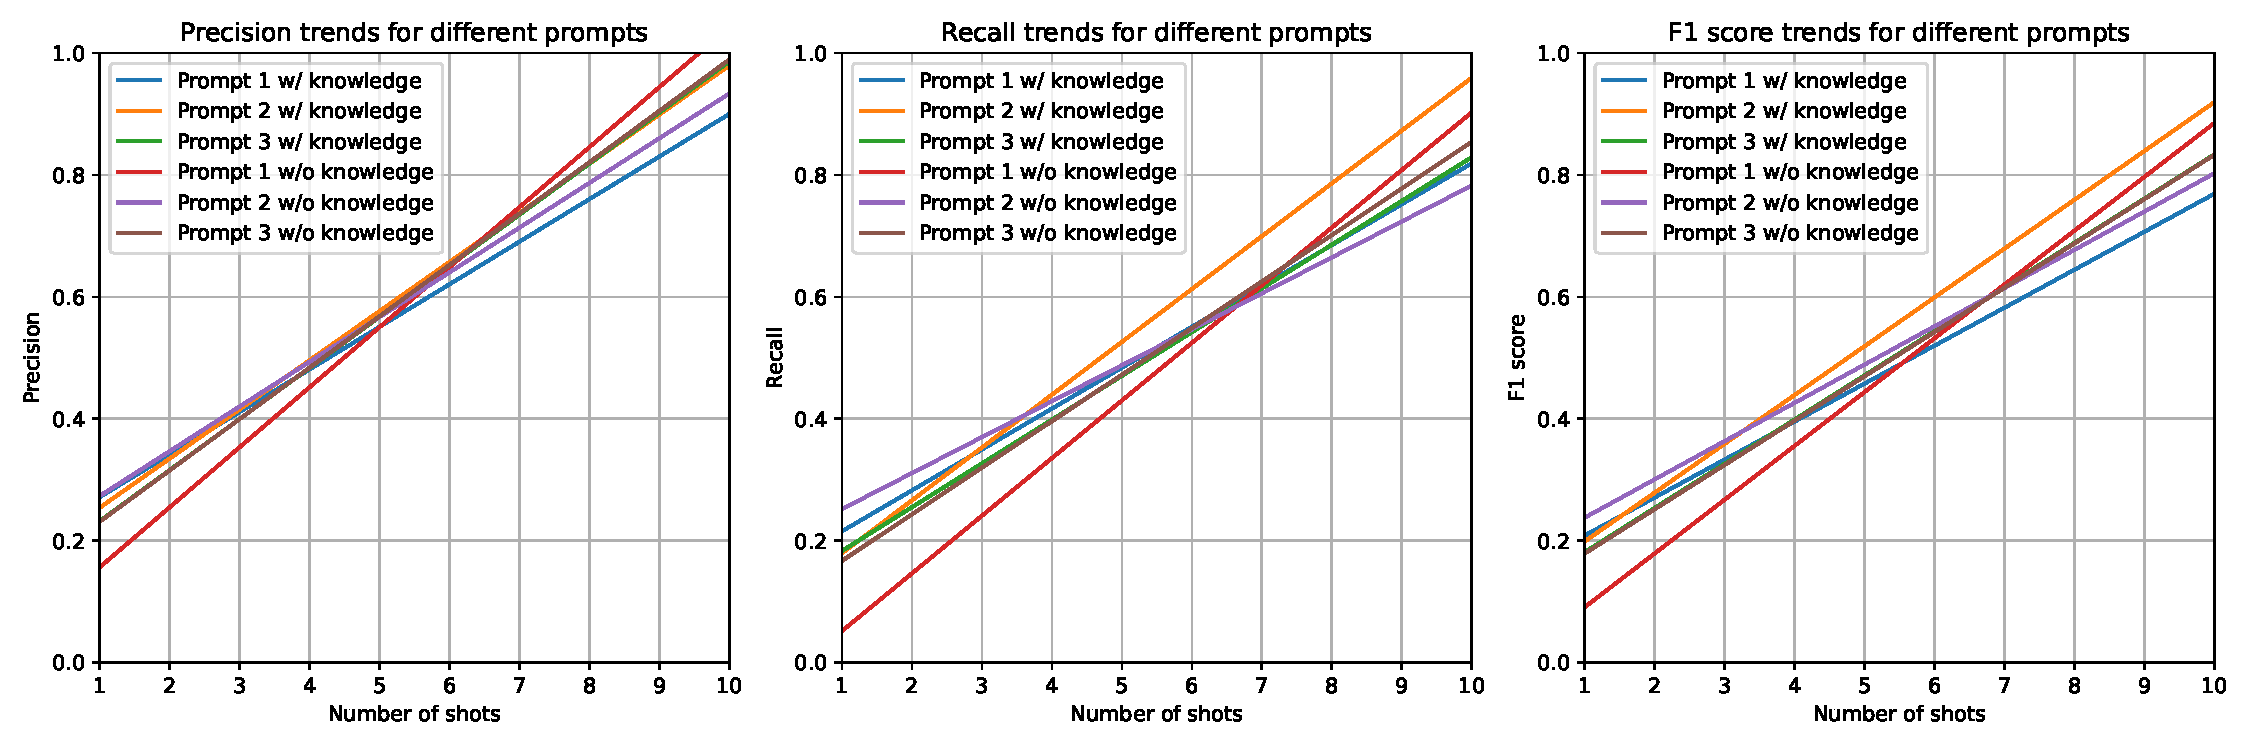
\includegraphics[width=\textwidth]{figures/specific_all_metrics_trend.pdf}
    \caption[Specific PDDL domain trend lines for precision, recall and F1 score]{Trend lines for precision, recall and F1 score with the three different prompts, with and without generated knowledge.}
    \label{fig:specific_all_metrics_trend}
\end{figure}

\begin{figure}[h]
    \centering
    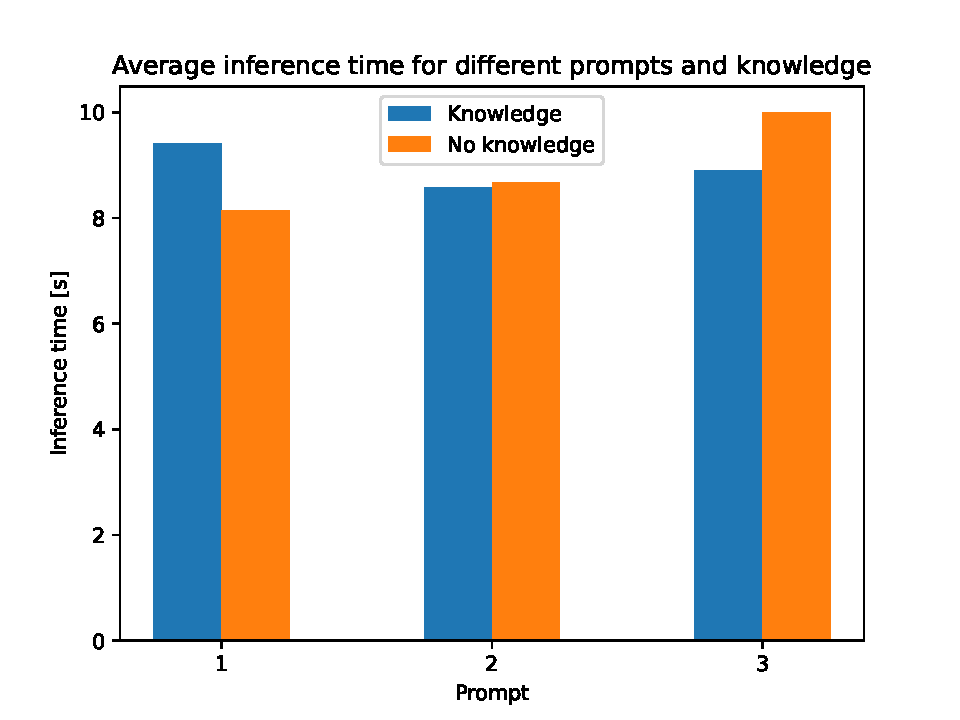
\includegraphics[width=0.6\textwidth]{figures/specific_avg_inf_time.pdf}
    \caption[Specific PDDL domain average inference time]{Comparison of average inference time for the specific PDDL domain tests with and without knowledge.}
    \label{fig:specific_avg_inf_time}
\end{figure}

\begin{figure}[h]
    \centering  
    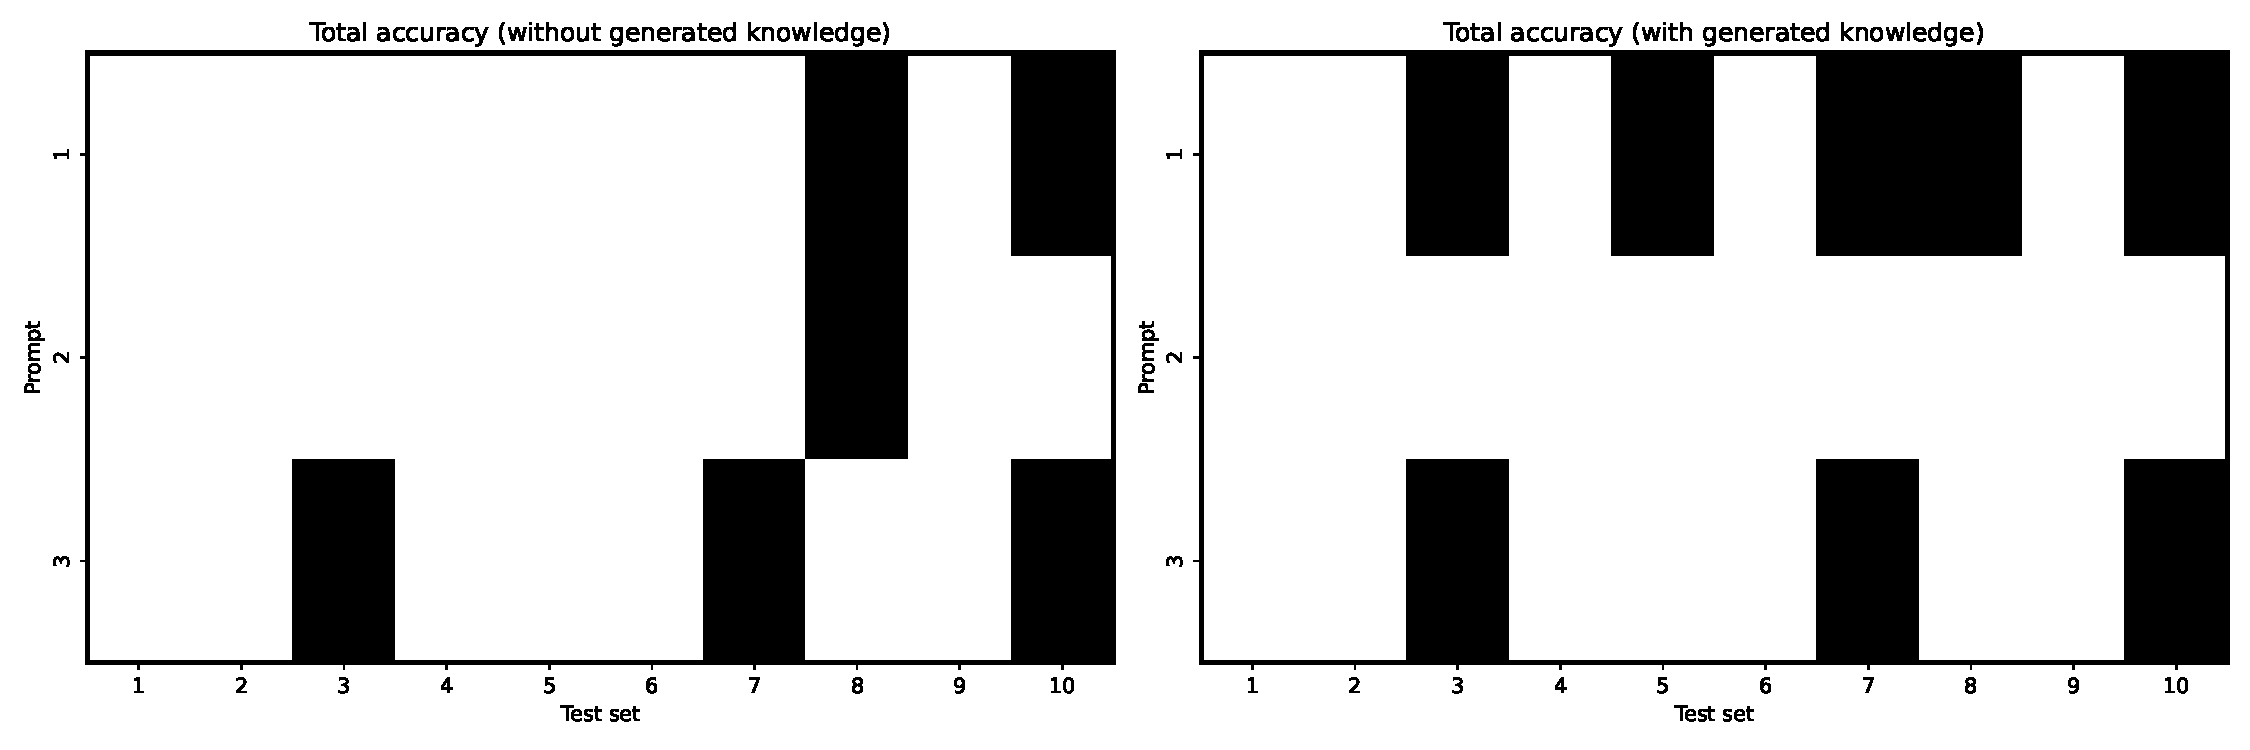
\includegraphics[width=0.9\textwidth]{figures/specific_heatmaps.pdf}
    \caption[Specific PDDL domain $\text{total}_{accuracy}$]{Heatmaps showing the $\text{accuracy}_{total}$ for all prompts with and without knowledge.}
    \label{fig:specific_heatmap}
\end{figure}

\section{POPF}\label{sec:POPF_experiments}
We tested POPF isolated from SemReBot2 and PlanSys2 by giving it a \verb|domain.pddl| and different
\verb|problem.pddl| files. The domain and problems were solely relevant to the SemReBot2 use case. We
checked 14 different scenarios one time each. As POPF is a deterministic AI planner, we only had to
check every scenario one time.

The scenarios ranged from simple navigation tasks to picking up one to 10 pallets and placing
them at different locations. We also checked the planner's ability to plan for battery capacity,
logical errors in the problem file, and its ability to plan the shortest possible path.

We created three different metrics, success rate $\eta_{success}$, time and battery efficiency, $\eta_{time}$ and $\eta_{battery}$, respectively, and planner time. $\eta_{success}$ is the average of how many times the planner creates a solvable plan, and time and battery efficiency is the ratio of the planner's output time and battery matched against an optimal answer created by us

\begin{equation}\label{eq:popf_metrics}
    0.00 \leq \eta_{success}, \eta_{time}, \eta_{battery} \leq 1.00
\end{equation}

Test no. 13 contained logical errors, meaning that the planner should not be able to create a solvable plan. For this test, if the success was "No", it would count as $1.00$ towards all metrics as the planner indeed managed to spot an error.

The planner time is the time it takes for POPF to create a plan once it receives the domain and the problem file.

As in the simulation environment, the distance and time taken between waypoints is computed dynamically, and the battery costs of each action are the same.

In all 14 tests, except Test 13, POPF managed to create a solvable plan. The results can be seen in Table \ref{tab:popf_metrics}

\begin{table}[]
\centering
% \resizebox{\textwidth}{!}
{%
\begin{tabular}{|l|l|l|l|}
\hline
\textbf{Avg. planner time} & $\mathbf{\eta}_{success}$ & $\mathbf{\eta}_{time}$ & $\mathbf{\eta}_{battery}$ \\ \hline
0.33                       & 1.00                      & 0.93                   & 0.95                      \\ \hline
\end{tabular}%
}
\caption[POPF experiment results]{POPF average inference time and experiment metrics.}
\label{tab:popf_metrics}
\end{table}

For planner time, $\eta_{time, i}$ and $\eta_{batter, i}$ per test, see Figure \ref{fig:popf_metrics}.

\begin{figure}
    \centering
    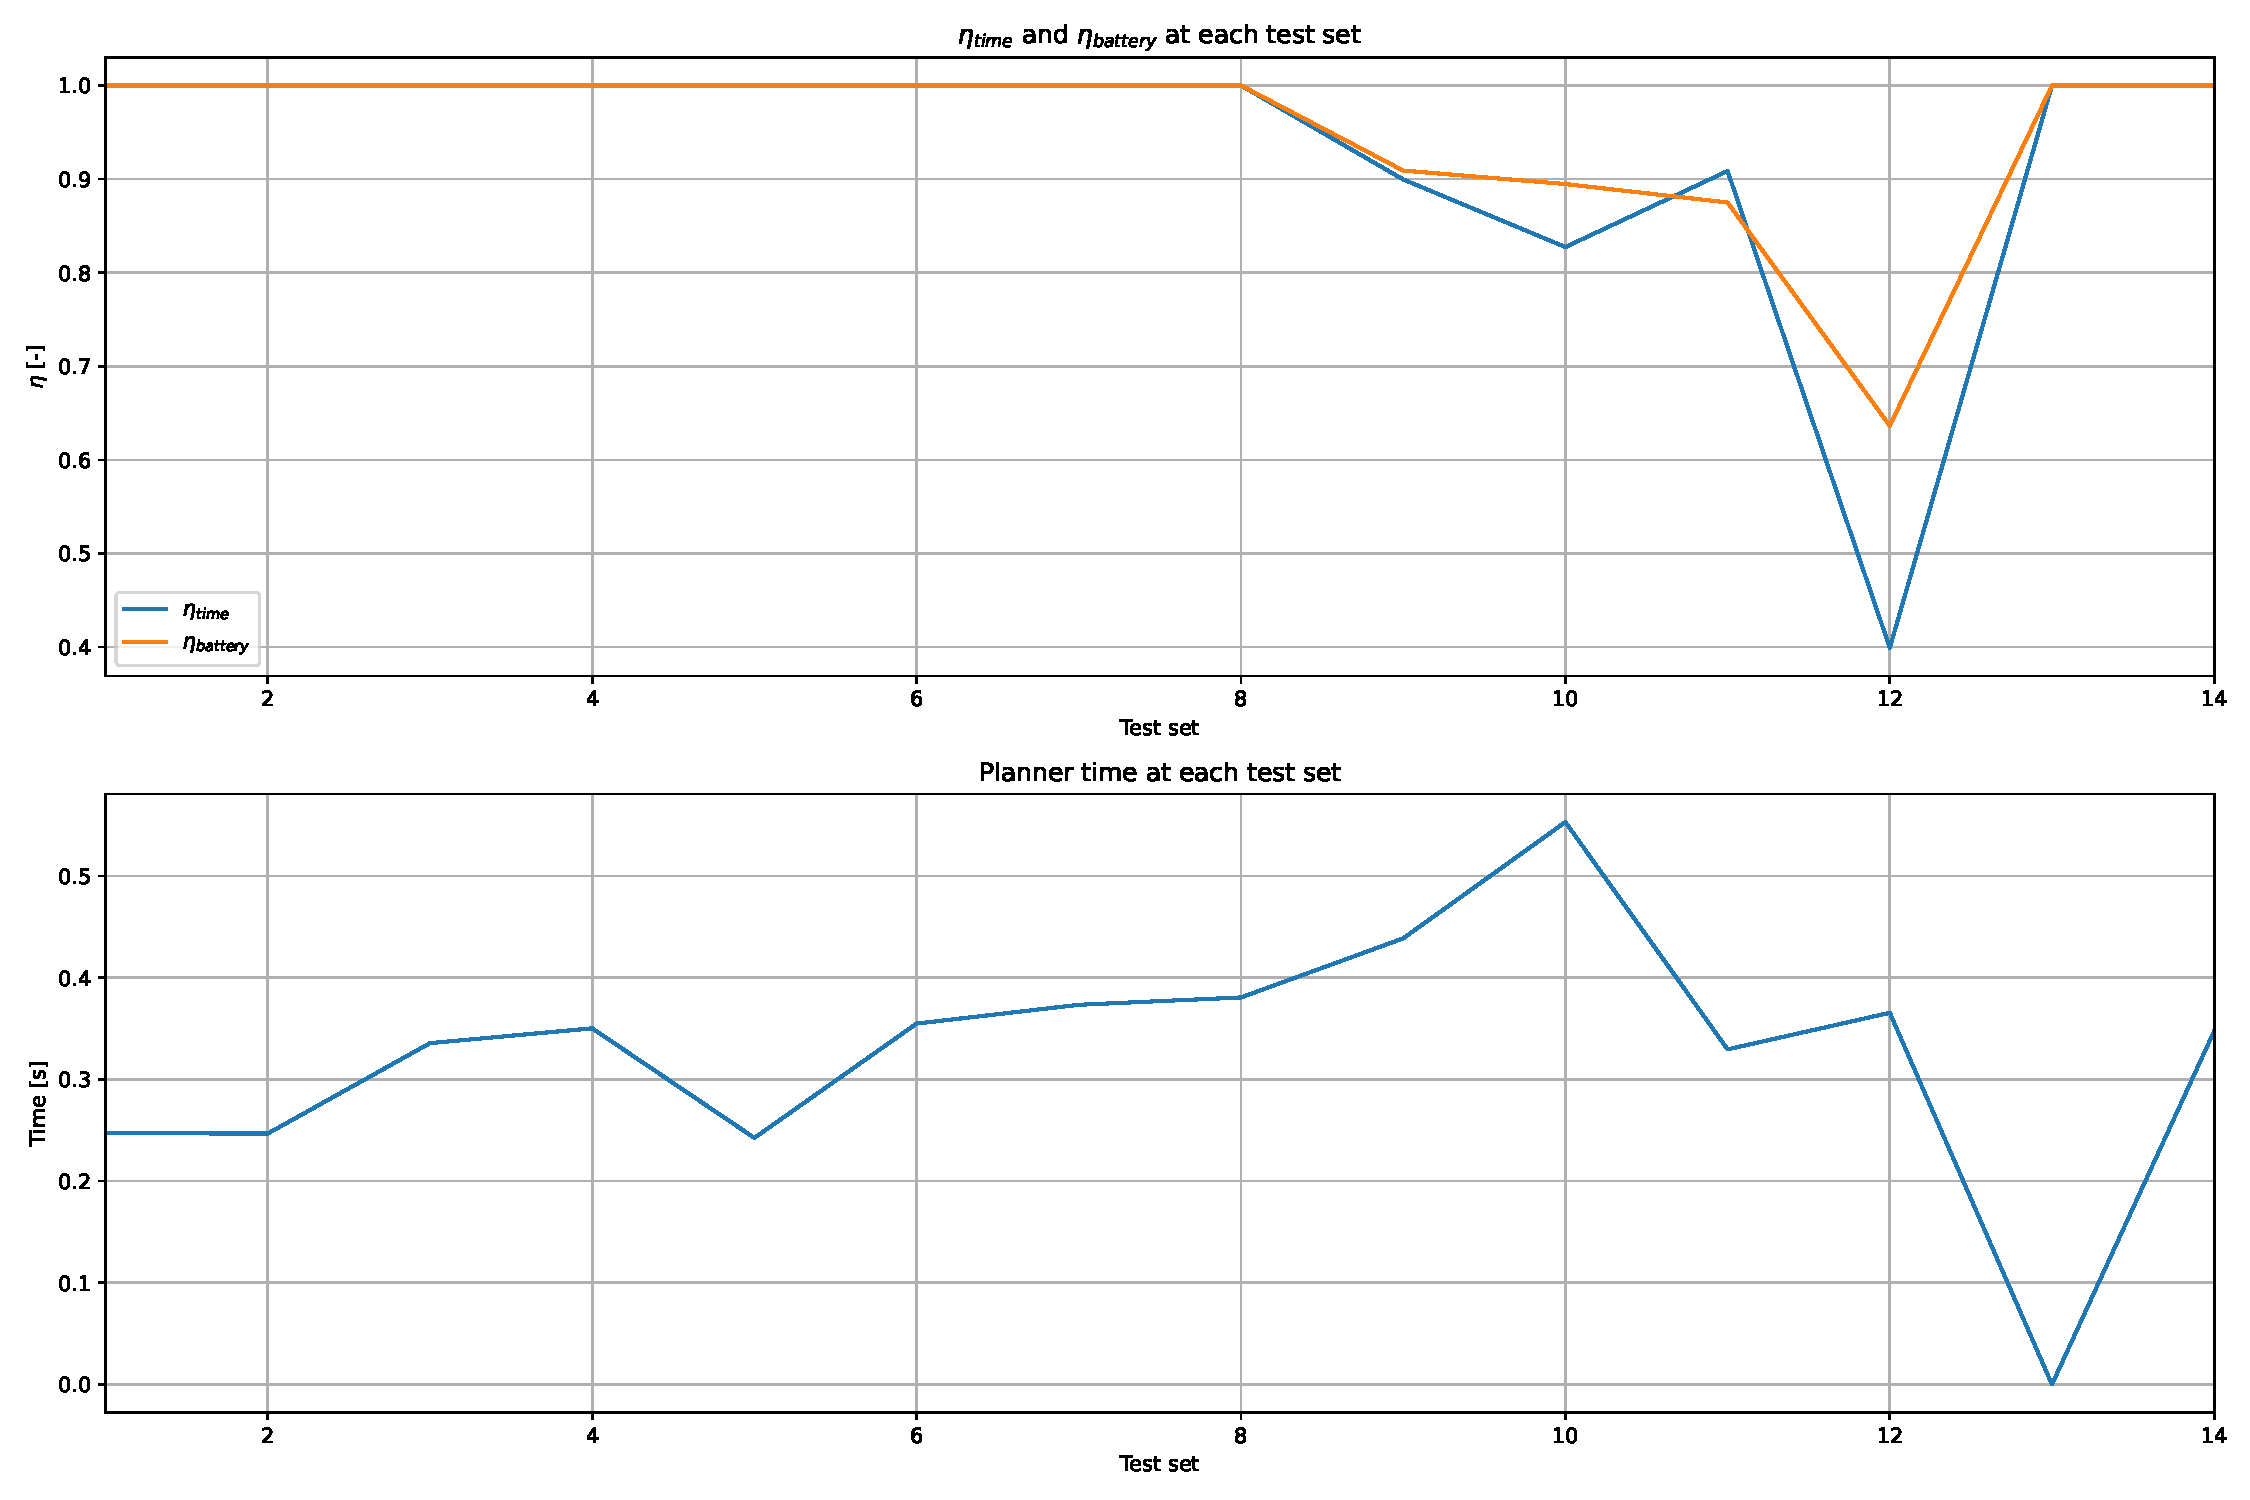
\includegraphics[width=\textwidth]{figures/popf_metrics.pdf}
    \caption[POPF metrics]{Planner time, $\eta_{time, i}$ and $\eta_{batter, i}$ change at each test.}
    \label{fig:popf_metrics}
\end{figure}

\section{SemReBot2 full system tests}\label{sec:SemReBot2_experiments}
For the full system test we provided SemReBot2 with four pre-recorded audio tracks containing one natural language command each. 